\cleardoublepage
\newpage
\ifdefined\EnableIncludeImages
    \ThisULCornerWallPaper{1.0}{chapterimage.eps}
\fi
\chapter*{Introdución} % 
\addcontentsline{toc}{chapter}{Introdución} %% Agregando manualmente a la tabla de contenidos

%% Usei a mesma estrutura do inicio do quijote
En mi querido pueblo de Occo, en la época de mi primera década, yo pasaba mis días dividiendo mi tiempo entre los trabajos de la chacra\footnote{También escrita como \textit{chakra}, esta es una palabra quechua que hace referencia a un terreno de cultivo.}, mis juegos infantiles e innumerables paseos por el campo.
Los trabajos de la chacra, aunque fuesen pesados para mí, eran posibles de realizar porque estaban divididos con toda la familia. 
Aun así, los días en el campo no transcurrían limpios de sorpresas, dado que, de cuando en cuando, alguno de nuestros animales se perdía; en esos casos, yo salía por las laderas de los montes llamándolo por su nombre hasta que escuchaba una respuesta, generalmente en forma de un lamento lleno de tristeza y añoranza.
Esa táctica era especialmente eficaz con mi burrito, pues él conseguía escuchar mi llamado aunque estuviera en otras montañas. Así, cuando yo gritaba su nombre, él volvía a mí gritando y llorando, escogiendo su camino en función de la dirección de mi voz.  
En otras ocasiones, percibíamos que desaparecían animales pequeños, como pollos o cuyes; sin embargo, después de observar las evidencias y hacer un trabajo ``detectivesco'', descubríamos que su ausencia era debido a la ``visita'' de algún halcón, zorro o gato de montaña.
En esos casos, nosotros solo podíamos llorar por ellos; no obstante, pocas eran las veces que perdíamos animales de esa forma, dado que, además de las personas de la casa, nosotros teníamos animales como perros y gatos que nos ayudaban a vigilar.

\ifdefined\EnableIncludeImages
\begin{wrapfigure}{r}{0.49\textwidth}
  \begin{center}
  \vspace{-20pt}
    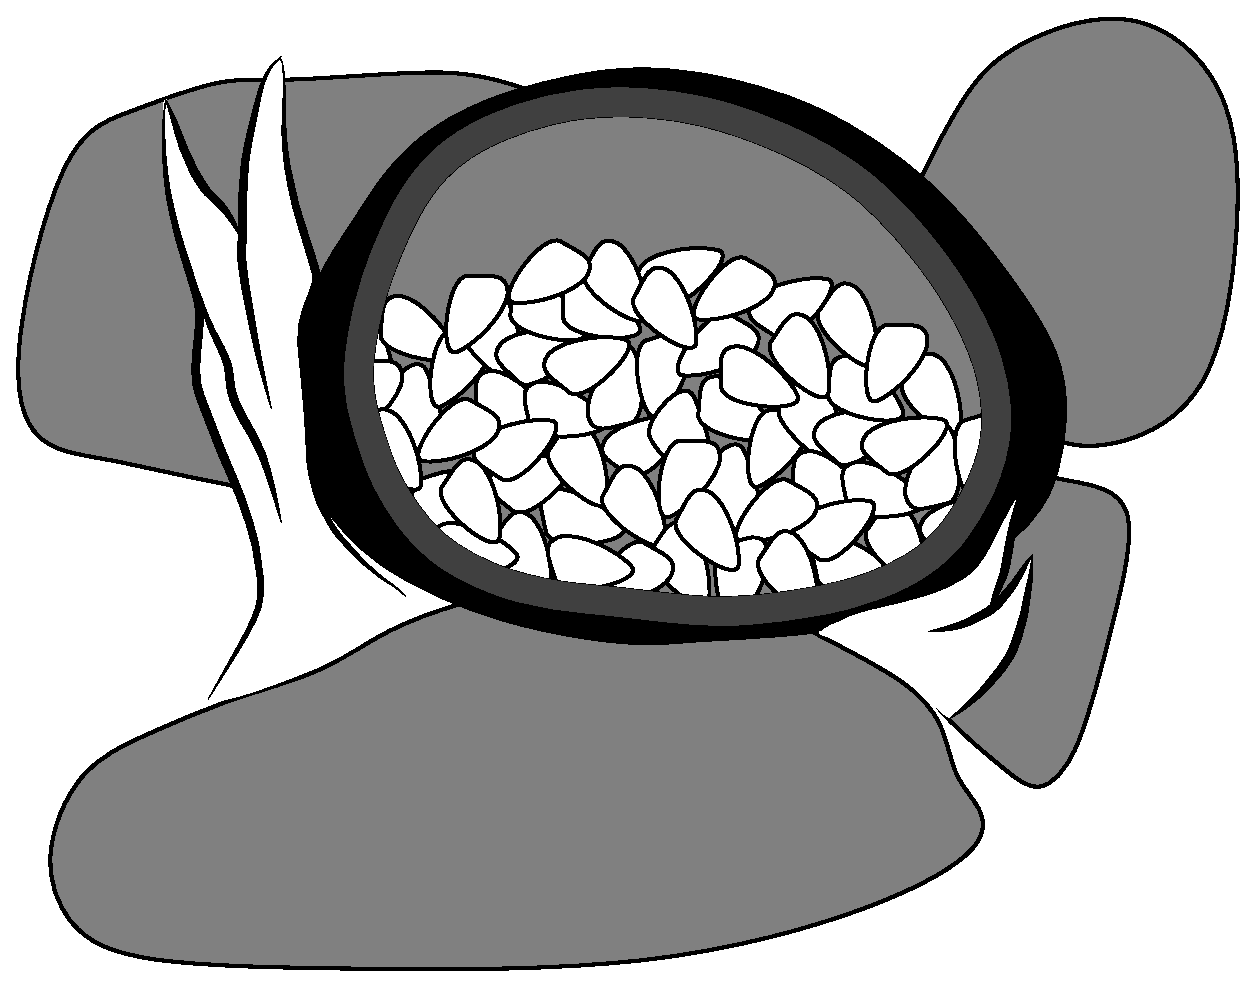
\includegraphics[width=0.47\textwidth]{cancha.eps}
  \end{center}
  \vspace{-20pt}
  %\caption{Zandor}
\end{wrapfigure}
\fi
Mi familia no era acomodada, y tal vez ese concepto escapaba a mi comprensión en aquella época, mas nada de lo que realmente importaba me faltaba.   
Recuerdo que mi casa era de adobe y madera, con techo de tejas, y mi mamá cocinaba nuestros alimentos sobre una pequeña fogata. Mis hermanas y yo, con mucha frecuencia, usábamos atuendos que, a simple vista, cualquier persona consideraría que eran varias medidas menores o mayores de las que realmente necesitábamos;
sin embargo, para mí y para mis hermanas, eso poco importaba. Mi casa era un castillo amplio y fresco al cual yo iba a descansar después de volver de la escuela o del trabajo en la chacra.
La comida de mi mamá era lo mejor del día, pues estaba llena de los sabores de los productos que nosotros mismos cultivábamos o cuidábamos. 
En días especiales, mi papá iba al río para pescar y comíamos pescado frito en el almuerzo. Otras veces, en época de sequía, comíamos charqui\footnote{Carne deshidratada al sol.}, con alguna mezcla de huevos de perdiz o de gallina, dependiendo de la suerte del día.
El queso y la leche no faltaban en nuestras comidas, que tanto podían ser de cabra como de vaca.
Los postres dependían de la estación del año, pues las frutas como tunas, duraznos, higos, sanky\footnote{Fruta del Ande peruano que tiene múltiples beneficios para la salud.}, entre otras, tenían cada una su temporada. También había épocas para sobremesas elaboradas con maíz fresco y otras con calabaza; con esta última, mi mamá hacía mi mazamorra favorita. Era increíble para mí que una crema de semejante majestad pudiese ser preparada con sólo un poco de dulce de molle\footnote{El \textit{molle} o \textit{Lithraea molleoides}, es un substituto del azúcar.}, canela, clavo de olor y calabaza\footnote{Calabaza o \textit{Cucurbita ficifolia}.}.

A mis hermanas y a mí nos gustaba jugar juntos, salir a pasear buscando frutas e ir a apreciar a los animales silvestres. En general, nosotros no teníamos discusiones importantes; sin embargo, debo reconocer que yo, de cuando en cuando, acostumbraba hacerles alguna travesura.
En esos casos, ellas recurrían a las máximas autoridades de la casa, con los señores que gobernaban y decidían sobre el bien y el mal, es decir, mis padres. 
Recuerdo que, al principio, mi papá me hablaba con frases como:\\\indent
---Aule, no debes esconder la muñeca de tu hermana.\\\indent
Si el asunto era más grave, él me decía: \\\indent
---¡Aurelio! ¿Por qué colocaste un grillo en la cabeza de tu hermana?\\\indent
Si mi insistencia en la búsqueda de problemas llegaba a niveles mayores, mi papá gritaba con energía:\\\indent
---¡Aulicha! ¿Por qué colocaste ají en el caramelo de tu hermana?\\\indent
Así, cuando yo escuchaba que mi papá me llamaba \textit{Aulicha}, yo ya sabía que mi suerte había sido decidida y que una chicoteada estaba próxima. La idea de huir siempre pasaba por mi cabeza; pero mis experiencias anteriores me indicaban que eso solamente iba a perjudicarme más e iba resignado delante de mi papá. Inclusive, en varias ocasiones, él me pedía que le alcanzara ese chicote de tres puntas, pequeño y veloz, que era al mismo tiempo un viejo conocido y mi principal antagonista. 
Sin embargo, después del castigo y pasado un tiempo, aproximadamente de media hora,
él me buscaba para consolarme y abrazándome decía:\\\indent
---¿Por qué te portas así? No debes molestar a tu hermana... pórtate bien.

Mi vida en el campo siempre estaba llena de contrapuntos, tantos eran los momentos tristes como los alegres, y  algunas veces, más de las que me permitirían pensar que era solo una casualidad, los momentos tristes preparaban un camino inevitable e irreversible a épocas alegres y viceversa; como un ciclo que se retroalimenta para mantenerse perpetuo.
Así, una de mis mayores alegrías era saber que mi papá retornaba de viaje, generalmente de la costa del Perú, no solo debido a la tristeza y la añoranza que dejaba su partida y la alegría que traía su retorno, sino también porque él volvía lleno de regalos. 
Nos traía dulces, galletas, juguetes, ropas, entre otros, a los cuales, comúnmente, nosotros en los Andes no teníamos acceso.
Por otro lado, entre mis momentos más tristes, estaba la pérdida de algún ser querido y la consecuente impotencia al no ser capaz de evitar su partida.
No obstante, todo eso es parte de la vida y me gustaría compartir con ustedes algunos de esos momentos.





%Ayacucho é uma cidade do distrito de Ayacucho, na província de Huamanga, no departamento de Ayacucho, no Peru
